%!TEX root = main.tex

\chapter{Probability}
\label{chapter:probability}

To develop a robust understanding of statistics, it is critical to understand
basic concepts in probability theory. Probability theory is an entire branch of mathematics, and a very complicated one. Here I will give only the essentials as
they have a direct bearing on statistics. I will leave many things out; what you
see here is not a complete theory of probability.

\section{Probability has at least two definitions}

We think about probability every day, for example, for
prediction. Given the weather report, is it worth it for me to carry an
umbrella? As a practicing scientist, you might ask yourself a different
kind of question every day: given the results of my experiments, how
likely is it that my hypothesis is correct?

For such a familiar concept, probability is actually very philosophically
thorny, and there are multiple \emph{interpretations} of the concept of
probability. Our intuitive sense of probability mostly aligns with the
\emph{Bayesian} interpretation, under which \emph{probability} refers to
a sense of confidence
about an unknown thing, often a future event. If I say the probability of an
event is 1\%, it means, in a practical sense, that I'm willing to bet a fair
amount of money it won't happen. Philosophically, it's hard to say what ``1\%
confident'' really means, but the concept should be very intuitive.

Unfortunately, Bayesian statistics is mathematically and technically
challenging. It also requires an assertion of a \emph{prior probability}: you
must state the probability that your hypothesis was true before you started the
experiment. The apparent subjectivity of prior probabilities was repugnant to
some early, prominent statisticians, who mostly directed the field of statistics
away from the Bayesian interpretation and toward the \emph{frequentist}
interpretation of probability.

In the \emph{frequentist} interpretation, the probability of an outcome is
the proportion, or frequency, of a that outcome when a trial is repeatedly
many times. To say there is a 50\% probability of flipping a coin and seeing heads
means that, as you flip the coin over and over again, the proportion of
flips that come up heads will approach 50\%.

For technical, philosophical, and historical reasons, when we talked about
``statistics'' with no modifier, we mean frequentist statistics. For better
or worse, frequentist is the default; Bayesian is the exception.

\section{A frequentist interpretation cannot assign probabilities to states of nature}

A problem with the frequentist definition is that probabilities can only
be assigned to experiments or situations that can be repeated infinitely many
times. It does not make sense to ask about the probability that it will rain
tomorrow any more than it makes sense to ask about the probability than it makes
sense to ask about the probability that it rained yesterday: it either rained or
it didn't, either it will rain or it won't.

The fact that we live in just one universe means that, under the frequentist 
interpretation, you cannot ask about the probability of a state of nature.
Critically, you cannot ask about the probability your hypothesis is correct.
Your hypothesis is either correct or not, so the probability that it is correct
is either zero or one. You just don't know which of those two possibilities is
right!

As a scientist, this is deeply dissatisying.  The whole point of statistical
inference is to figure out what's going on in the world. I don't want to feed
my hard-won experimental data into a statistical algorithm that says, ``If your
hypothesis is true, then it is; and if it's not, it's not.''

Imagine that I show you a coin, then put my hands behind my back, and tell you
the coin is in one of my hands. I ask you, ``What is the probability the coin
is in my left hand?'' In the frequentist interpretation, probability is a fixed,
objective thing. The fact that you know less than me about where the coin's
location is irrelevant; the fact that the coin truly is in one hand or the other
is all the frequentist interpretation knows.

The Bayesian approach is more appealing in that it does in fact allow you to
ask about the probability of states of nature. There is such a thing as a
Bayesian probability that it will rain tomorrow or that your scientific
hypothesis is correct. In a Bayesian interpretation, where
probability can be subjective, it is OK that I put the probability of the coin
being in my left hand as 0\% or 100\%, even while you assign the probability as
just 50\%. Nevertheless, we will pursue a frequentist interpretation here.


\section{Probability is a function}

The frequentist definition of probability has to do with the
proportions of infinitely-repeatable trials that have some \emph{outcome}. An
outcome is any thing that can happen as a result of an infinitely-repeatable
trial. For example, if you flip a coin, you will get heads, or you will get
tails.

The \emph{sample space}, written $\Omega$, consists of all outcomes as well as
all possible combinations of outcomes. A combination of outcomes is called an
\emph{event} and written $\omega$. In other words, outcomes are individual,
real things that might happen, while events are abstract groupings of
outcomes. The sample space is the set of all events, which includes outcomes.

In the context of flipping a coin, ``flipped
heads'' is an outcome and an event. The empty set $\varnothing$ (``nothing
happened'') and the set of all outcomes $\Omega$ event (``something happened'')
are both events, but they are not outcomes. Some other examples of outcomes,
events, and sample spaces are in Table \ref{tab:outcome-event}. 

\begin{table}
\centering
\begin{tabular}{p{3cm}p{4cm}p{6cm}}
\toprule
Situation & Outcomes & Events \\
\midrule
Flipping a coin & heads ($H$), tails ($T$) & $\varnothing$, $H$, $T$, $\Omega$ \\
Rolling a die & $1, 2, \ldots, 6$ & $\varnothing$; the outcomes $1, 2, \ldots, 6$; $\binom{6}{2}$ 2-event outcomes (e.g., 1 or 2); $\binom{6}{3}$ 3-outcome events (e.g., 1, 2, or 3); $\ldots$; $\binom{6}{5}$ 5-outcome events (e.g., any except 1); $\Omega$ \\
Drawing a card & 2 of Clubs, $\ldots$, Ace of Hearts & $\varnothing$; the 52 outcomes (e.g., 2 of Clubs); $\binom{52}{2}$ 2-outcome events (e.g., a black Ace); $\ldots$; $\binom{52}{51}$ 51-outcome events (e.g., any card except 2 of Clubs); $\Omega$ \\
Pick a random decimal number between 0 and 1 & All real numbers between 0 and 1 & $\varnothing$; intervals like $[0, \tfrac{1}{2}]$; ``all subsets'' of $[0, 1]$; $\Omega$ \\
Your experiment & Each possible configuration of atoms at the moment of measurement & ``Cancer cell died'', ``Electron had energy between 1 and 2 eV'', etc. \\
\bottomrule
\end{tabular}
\caption{Example distinctions between outcomes and events.}
\label{tab:outcome-event}
\end{table}

As an aside, I note that defining ``all possible subsets of outcomes'' is
straightforward for a discrete case like flipping a coin or drawing a card, but
it is complicated for a continuous case like drawing a random real number
between $0$ and $1$. In continuous cases, a rigorous definition for the event
space $\Omega$ requires concepts from \emph{measure theory}, including a
$\sigma$-\emph{algebra}. I avoid these complexities in this chapter at the cost
of presenting a mathematically incomplete theory of probability.

The \emph{probability function} $\mathbb{P}$ maps events to numbers between $0$ and $1$:
\begin{equation*}
\mathbb{P} : \Omega \to [0, 1]
\end{equation*}
For example, if $H$ is the event of flipping heads, then $\prob{H} =
\tfrac{1}{2}$. I use the square brackets to emphasize that $\mathbb{P}$ is a
function of something other than numbers: $H$ is not a number like $5$, it is
an \emph{event}, a distinct mathematical object.

Basic axioms of probability theory require that, for any probability function,
the probability that ``nothing happened'' is zero and the probability
that ``something happened'' is one:
\begin{align*}
\prob{\varnothing} &= 0 \\
\prob{\Omega} &= 1
\end{align*}

\section{``Or'' adds event probabilities; ``and'' multiplies}

The axioms about probability functions also mean that there are specific rules
around manipulating probabilities. For example, we're often interested in the
relationships between events. What is that probability that this \emph{or} that
happened? What is the probability that this \emph{and} that happened?

If $A$ and $B$ are two events that don't have any constituent outcomes in
common, we call then \emph{disjoint}, and their probabilities add. For example,
the probability of flipping a heads \emph{or} flipping a tails is the
probability of heads plus the probability of tails.  Mathematically we write
this as
$$
\text{if } A \cap B = \varnothing \text{, then } \prob{A \cup B} = \prob{A} + \prob{B},
$$
where the ``cap'' $\cap$ means \emph{intersection} (``and'') and the ``cup'' $\cup$ means
\emph{union} (``or''), so this reads ``if no outcomes are in both events $A$ and $B$,
then the probability of $A$ or $B$ is the sum of their individual probabilities.''

If $A$ and $B$ do have some overlap, you need to subtract out the probability
of the overlap. For example, consider drawing a card
from a standard 52-card deck. What is the probability of drawing a Jack \emph{or} a
Diamond? If you add up the probability of drawing a Jack and the probability
of drawing a Diamond, you end up double-counting the Jack of Diamonds event.
The solution is to subtract out the double-counted event:
$$
\prob{A \cup B} = \prob{A} + \prob{B} - \prob{A \cap B}.
$$

If ``or'' adds probability, how do we
find the probability of $A$ and $B$? Say I flip two coins. What's the
probability that I flip heads on the first coin \emph{and} tails on the second?
If $A$ and $B$ are \emph{independent} events, then their probabilities
multiply. The probability of flipping a heads then a tails is $\tfrac{1}{2} \times
\tfrac{1}{2} = \tfrac{1}{4}$. (The probability that I flip heads and tails on
the \emph{same} flip is zero, since
$\mathbb{P}[H \cap T] = \mathbb{P}[\varnothing] = 0$.)

\section{Independence and conditional probability}

Mathematically, $A$ and $B$ are independent if and only if their probabilities
multiply. This might feel circular, so I will show you the logic.

Intuitively, two events are independent if they do not depend on each other. If
I flip two separate coins, or I flip the same coin twice, the one flip doesn't
affect the other flip.

It turns out that the simple phrase ``depends on'' produces deep philosophical questions.
Just as ``probability'' had frequentist and Bayesian definitions, so there are
multiple definitions of \emph{conditional probability}. The easiest
definition is:
\begin{equation*}
\prob{A | B} \defeq \frac{\prob{A \cap B}}{\prob{B}},
\end{equation*}
where $\prob{A | B}$ is pronounced ``the probability of $A$ given $B$''.

Although the definition of conditional probability is a mathematical axiom that
cannot be proven or disproven, it is easy to get an intuitive picture of why it
is chosen as an axiom. In a frequentist interpretation of probability, $\prob{A
| B}$ is, on a denominator of the trials in which $B$ happened, the proportion
of trials in which $A$ also happened. Say $n_B$ is the number of trials in
which $B$ happened, $n_{AB}$ is the number of trials in which $A$ and $B$
happened, and $n$ is the total number of trials. Then the proportion we're
talking about is $n_{AB} / n_B$, which corresponds to $\prob{A \cap B} /
\prob{B}$. I like to think of conditional probability as ``zooming in'' to a
smaller sample space: rather than thinking about all of $\Omega$, we are
thinking only about the subset of outcomes $\omega$ where $B$ happened (Figure
\ref{fig:conditional-probability}).

\begin{figure}
\centering
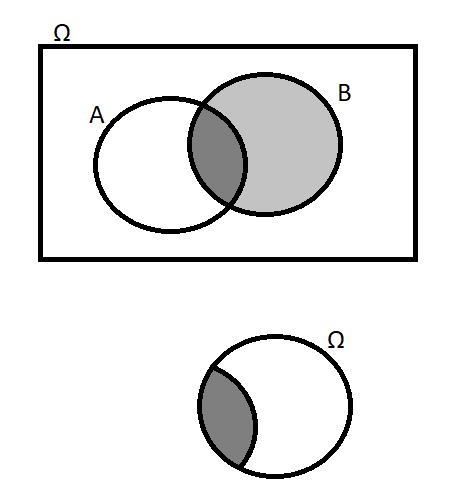
\includegraphics[]{figure/conditional-probability.png}
\caption{Conditional probability as shrinking of universe. To find $\mathbb{P}[A|B]$,
we imagine that $B$ is the entire sample space and consider the probability of
$A \cap B$ in that space.}
\label{fig:conditional-probability}
\end{figure}

If $A$ and $B$ are independent, then $A$ does not ``depend on'' $B$: the
probability of $A$ given that $B$ happened is equal to the probability of $A$
without knowing anything about $B$: if $A$ and $B$ are independent, then
$\prob{A | B} = \prob{A}$, and thus $\prob{A \cap B} = \prob{A} \times
\prob{B}$.

Given these rules, you can compute the probability of things like particular poker
hands.